\begin{figure}[htpb]
	\begin{center}
		\begin{tikzpicture}[scale=0.45, transform shape]

			\foreach \x in {0}{
				\node[draw, rectangle, fill=gray!10, minimum size = 0.4] (a\x) at (\x*8,8) {$T(n)$};
				\foreach \y in {0,...,2}{
					\node[draw,rectangle, fill=gray!10, minimum size =0.4] (b\y) at (-4+\x*8+\y*4,6) {$T(n/b)$};
					\draw (a\x) -- (b\y);
					\draw[dotted] (-6,7) -- node[fill=white] {$a$ calls} (6,7);
					\only<2->{
						\foreach \z in {0,...,2}{
							\ifthenelse{\y = 1}{
								\node[] (c\z) at (-1.5+\z*1.5,4.8) { };
								\draw[dashed] (b\y) -- (c\z);
								}{
								\node[draw,rectangle, fill=gray!10, minimum size =0.4] (c\z) at (-6+\x*8+\y*4+\z*2,4) {$T(n/b^2)$};
								\draw (b\y) -- (c\z);
								\foreach \a in {0,...,2}{
									\node[] (d\a) at (-6.5+\x*8+\y*4+\z*2+\a*0.5,2) { };
									\draw[dashed] (c\z) -- (d\a);
								}
							}
							\draw[dotted] (-5.5+\x*8+\y*4,5) -- node[fill=white] {$a$ calls} (-6+\x*8+\y*4+3.5,5);
						}
					}
				}
			}
			\node at (14, 0) { };

			\only<3->{
				\draw[fill=blue!60] (-8,2) rectangle node {$T(n/b^k)$} (7,3);
			}

			\only<4->{
				\foreach \x in {0,...,4}{
					\node[] (b\x) at (-7+\x*3,2) { };
					\node[draw, rectangle, fill=gray!10, minimum size = 0.4] (a\x) at (-8+\x*3,1) {$T(1)$};
					\draw[dotted] (b\x) -- (a\x);
				}

				\foreach \x in {0,...,4}{
					\node[] (b\x) at (-7+\x*3,2) { };
					\node[] (a\x) at (-7+\x*3,1) { };
					\draw[dotted] (b\x) -- (a\x);
				}

				\foreach \x in {0,...,4}{
					\node[] (b\x) at (-7+\x*3,2) { };
					\node[draw, rectangle, fill=gray!10, minimum size = 0.4] (a\x) at (-6+\x*3,1) {$T(1)$};
					\draw[dotted] (b\x) -- (a\x);
				}
			}

			\only<5->{
				\node at (9,9) {\Large Amount of nodes $\cdot$ combining};
				\node at (9,7.9) {\Large $1 \cdot f(n)$};
				\node at (9,5.9) {\Large $a \cdot f(n/b)$};
				\node at (9,3.9) {\Large $a^2 \cdot f(n/b^2)$};
			}

			\only<6->{
				\node at (9,2.3) {\Large $a^k \cdot f(n/b^k)$};
				\node at (9,1.2) {\Large $a^{\log_b n } \cdot f(1)$};
			}

			\only<7->{
				\draw (7,0.5) -- (11,0.5) node[anchor = west] {\Large $+$};
				\node at (9,-0.2) {\Large $\sum\limits_{i=0}^{log_b n} a^i \cdot f(\dfrac{n}{b^i})$};
			}

			\only<8->{
				\node[anchor=west] at (-7, -0.2) {\Large Total time spent in the leaves: $\Theta(a^{\log_b n}) = \Theta(n^{\log_b a})$.};
			}

			\only<9->{
				\node[red, anchor=west] at (5, -0.2) {\Large $\leq, =, \geq$};
				\node[red, anchor=west] at (4.7, -1.2) {\Large Which is it?};
			}

		\end{tikzpicture}
	\end{center}
\end{figure}
